%Notes by Harsh Mistry 
%CS 350
%Based on Template From  https://www.cs.cmu.edu/~ggordon/10725-F12/template.tex

\documentclass[twoside]{article}
\setlength{\oddsidemargin}{0.25 in}
\setlength{\evensidemargin}{-0.25 in}
\setlength{\topmargin}{-0.6 in}
\setlength{\textwidth}{6.5 in}
\setlength{\textheight}{8.5 in}
\setlength{\headsep}{0.75 in}
\setlength{\parindent}{0 in}
\setlength{\parskip}{0.1 in}
\usepackage{amsmath,amsfonts,graphicx}
\newcounter{lecnum}
\renewcommand{\thepage}{\thelecnum-\arabic{page}}
\renewcommand{\thesection}{\thelecnum.\arabic{section}}
\renewcommand{\theequation}{\thelecnum.\arabic{equation}}
\renewcommand{\thefigure}{\thelecnum.\arabic{figure}}
\renewcommand{\thetable}{\thelecnum.\arabic{table}}
\newcommand{\lecture}[4]{
   \pagestyle{myheadings}
   \thispagestyle{plain}
   \newpage
   \setcounter{lecnum}{#1}
   \setcounter{page}{1}
   
   \graphicspath{ {images/} }
   
%Info Box 
   \begin{center}
   \framebox{
      \vbox{\vspace{2mm}
    \hbox to 6.28in { {\bf CS 350 - Operating Systems
	\hfill Winter 2018} }
       \vspace{4mm}
       \hbox to 6.28in { {\Large \hfill Lecture #1: #2  \hfill} }
       \vspace{2mm}
       \hbox to 6.28in { {\it Lecturer: #3 \hfill Notes By: #4} }
      \vspace{2mm}}
   }
   \end{center}
   
   \markboth{Lecture #1: #2}{Lecture #1: #2}



 
}

\renewcommand{\cite}[1]{[#1]}
\def\beginrefs{\begin{list}%
        {[\arabic{equation}]}{\usecounter{equation}
         \setlength{\leftmargin}{2.0truecm}\setlength{\labelsep}{0.4truecm}%
         \setlength{\labelwidth}{1.6truecm}}}
\def\endrefs{\end{list}}
\def\bibentry#1{\item[\hbox{[#1]}]}

\newcommand{\fig}[3]{
			\vspace{#2}
			\begin{center}
			Figure \thelecnum.#1:~#3
			\end{center}
	}

\newtheorem{theorem}{Theorem}[lecnum]
\newtheorem{lemma}[theorem]{Lemma}
\newtheorem{ex}[theorem]{Example}
\newtheorem{proposition}[theorem]{Proposition}
\newtheorem{claim}[theorem]{Claim}
\newtheorem{corollary}[theorem]{Corollary}
\newtheorem{definition}[theorem]{Definition}
\newenvironment{proof}{{\bf Proof:}}{\hfill\rule{2mm}{2mm}}
\newcommand\E{\mathbb{E}}


%Start of Document 
\begin{document}

\lecture{2}{January 10, 2018}{Lesley Istead}{Harsh Mistry}

\section{Threads and Concurrency Continued}
\section{Implementing Concurrent Threads}
\begin{itemize}
\item Option 1 : multiple processors, multiple cores, etc
\item Option 2 : time sharing
\begin{itemize}
\item multiple threads take turns on the same hardware 
\item rapidly switch from thread to thread so that all make progress 
\end{itemize} 
\end{itemize}


\section{Time-sharing and Context Switches}

\begin{itemize}
\item When timesharing, the switch from one thread to another is called a \textbf{context switch}
\item During a context switch : 
\begin{enumerate}
\item Decide which thread will run next
\item Save registers contents of current thread 
\item Load register contents of  next thread
\end{enumerate}
\item Thread context must be save/restored carefully, since thread execution continuously changes the context. 
\end{itemize}

\subsection{What Causes Context Switches?}
\begin{itemize}
\item Calls to \verb|thread_yield|
\item Calls to \verb|thread_exit|
\item Blocks via call to \verb|wchan_sleep|
\item \textbf{preempted} threads
\begin{itemize}
\item runnign thread \textbf{involuntarily } stops running
\end{itemize}
\end{itemize}

\begin{center}
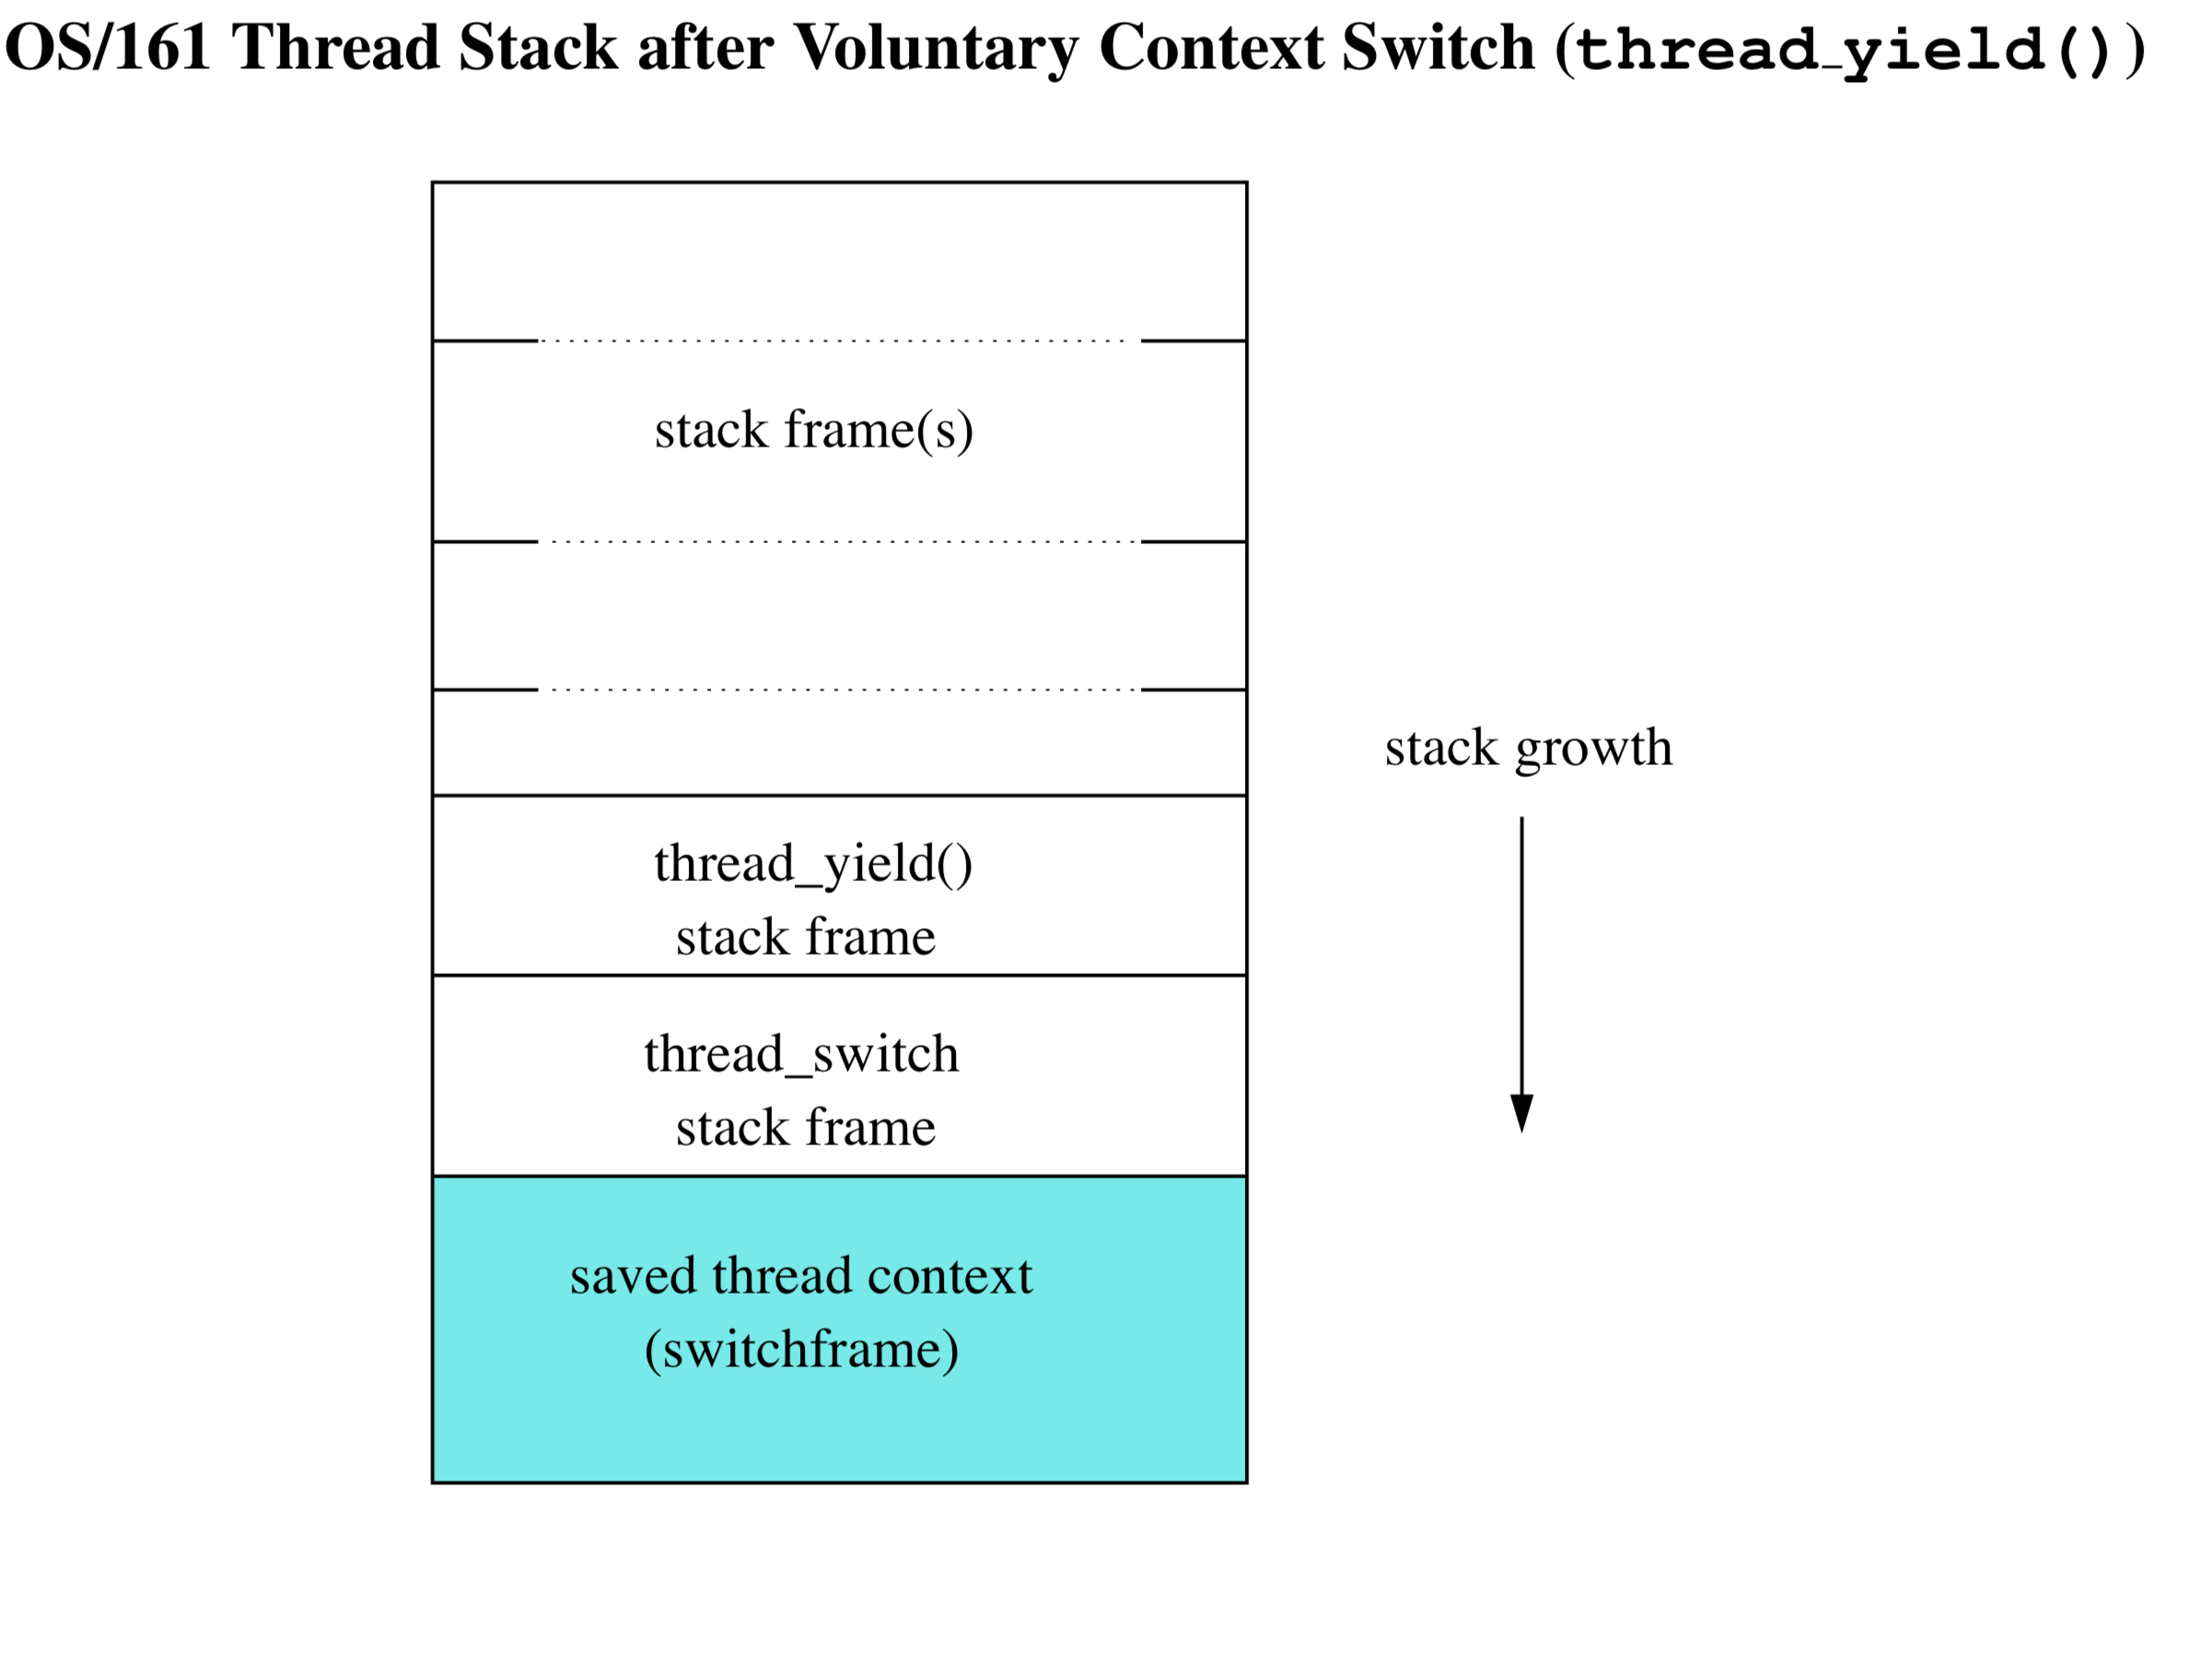
\includegraphics[scale=0.2]{2}\\12
Diagram taken from class slides 
\end{center}

\subsection{Preemption}
\begin{itemize}
\item \textbf{Preemption} prevents a running thread from potentially running forever 
\item \textbf{Preemption} means forcing a running thread to stop running, so that another thread can have a chance. 
\item To implement preemption, the thread library must have a means of "getting control" even though the running thread has not call a thread library function. This is normally accomplished using \textbf{Interrupts}
\end{itemize}

\subsubsection{Interrupts}
\begin{itemize}
\item An interrupt is an event that occurs during the execution of a program
\item Interrupts are caused by system devices
\item When an interrupt occurs, the hardware automatically transfers control to a fixed location in memory
\item At that memory location, the thread library places a pricedure called an \textbf{Interrupt handler}
\item The interrupt handler normally : 
\begin{enumerate}
\item Creates a \textbf{trap frame} to record context at the time of the interrupt 
\item Determines which device caused the interrupt and performs device-specific processing
\item Restores the saved thread context from the trap frame and resumes execution of the thread. 
\end{enumerate}
\end{itemize}

\subsubsection{Preemptive Scheduling}
\begin{itemize}
\item A preemptive scheduler imposes a limit, called the \textbf{scheduling quantum} on how long a thread can run before being preempted. 
\item The quantum is an \textbf{upper bound} on the amount of time that a threa can run. It may block or yield before its quantum has expired. 
\item Periodic timer interrupts allow running time to be tracked.
\item If a thread has run too long, teh timer interrupt handler preempts the thread by calling \verb|thread_yield|
\item The preempted thread changes state from running to ready, and its is placed on the ready queue. 
\end{itemize}

\begin{center}
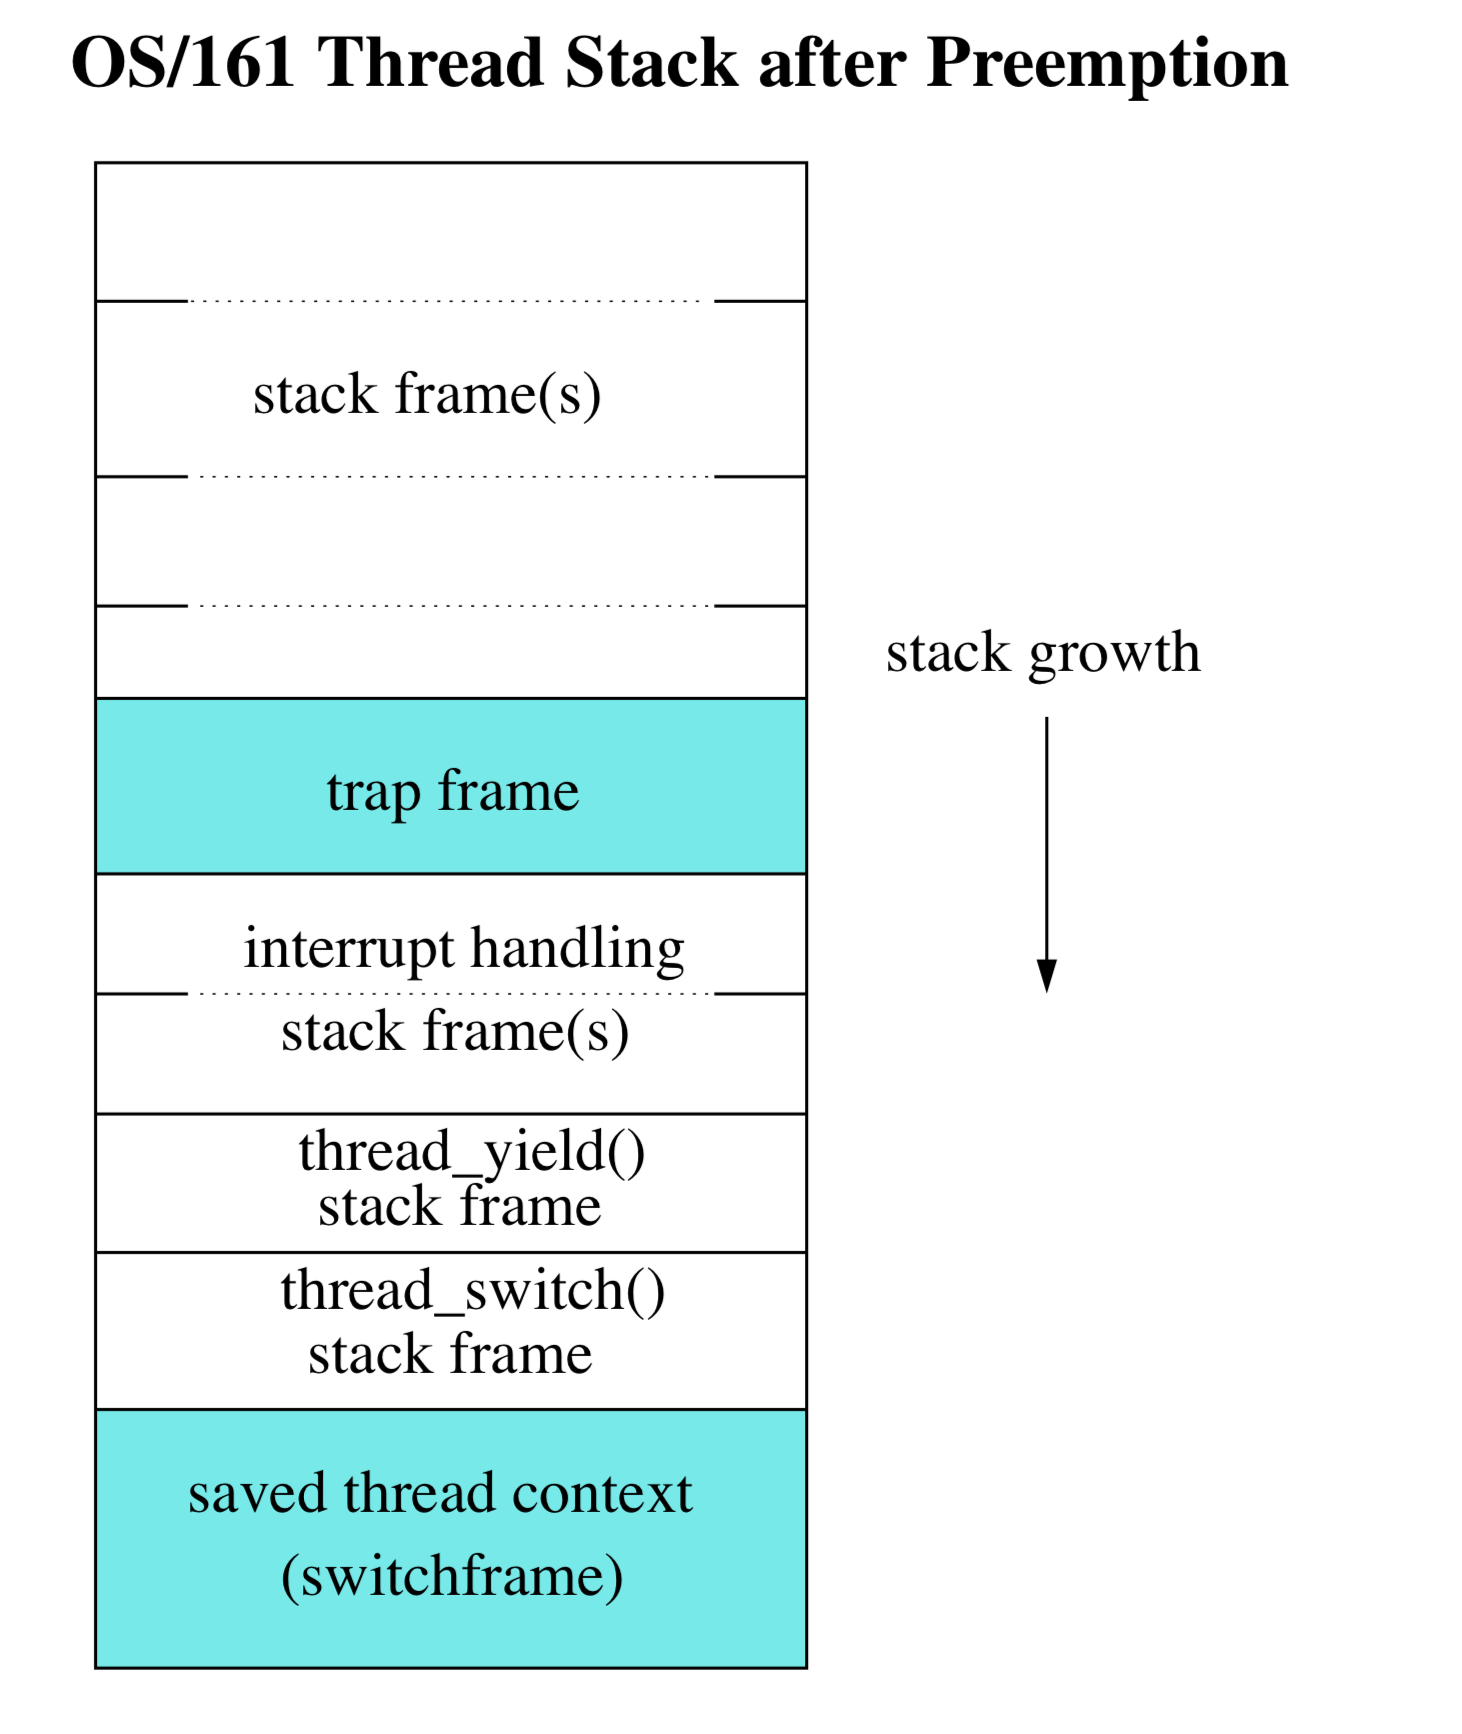
\includegraphics[scale=0.2]{3}\\
Diagram taken from class slides 
\end{center}

\end{document}


